% ============================================================
% CORRECTIONS (mai 2025) -- compatibilite TeX Live 2026
%   1. [francais]{babel} -> [french]{babel} (option deprecee, fatale avec LaTeX 2025-11+)
%   2. usepackage{graphicx} en double commente (deja charge avec [pdftex])
%   3. usepackage{float} commente (deja charge par le package algorithm)
% ============================================================
%---------Classe du document : book :-------------------%

\documentclass[a4paper,11pt,twoside,openright,notitlepage]{book}
\pdfobjcompresslevel 0
\usepackage[a-1b]{pdfx}


\makeatletter
\def\bstctlcite{\@ifnextchar[{\@bstctlcite}{\@bstctlcite[@auxout]}}
\def\@bstctlcite[#1]#2{\@bsphack
 \@for\@citeb:=#2\do{%
   \edef\@citeb{\expandafter\@firstofone\@citeb}%
   \if@filesw\immediate\write\csname #1\endcsname{\string\citation{\@citeb}}\fi}%
 \@esphack}
\makeatother

%-----------Package ------------------------------------%

\usepackage[french]{babel}
\usepackage[utf8]{inputenc}
\usepackage[T1]{fontenc}			
\usepackage{lmodern}
\usepackage{amsmath}					
\usepackage{amssymb}
\usepackage{units}				
\usepackage{amstext}        
\usepackage{amsfonts}        
\usepackage{theorem}          
\usepackage{array}						 
\usepackage{multicol}					
\usepackage{multirow}
\usepackage{lscape}
\usepackage{xspace}						
\usepackage[pdftex]{graphicx}	
\usepackage{subcaption}
\usepackage{indentfirst} 			
\usepackage{latexsym}					
\usepackage{setspace}					
\usepackage{algorithm}				
\usepackage{algorithmic}			
\usepackage{makeidx}					
\usepackage{vmargin}					
% \usepackage{float}  % déjà chargé par algorithm
\usepackage{enumerate}        
\usepackage{verbatim}         
\usepackage{floatflt}         
\usepackage{rotating}					
\usepackage{longtable}        
\usepackage[french]{varioref} 
%\usepackage{natbib}
\usepackage{diagbox}        
\usepackage{url}
\usepackage{pdfpages}           
\usepackage{titlesec} 
% \usepackage{graphicx}
\usepackage{minitoc}
\usepackage{xcolor,lipsum}
\usepackage[framemethod=tikz]{mdframed}
%\usepackage[maxnames=6,style=authoryear, style=ieee,backend=bibtex]{biblatex}
%\addbibresource{biblio.bib}
%\bibpunct{[}{]}{;}{a}{ }{,}

%------Page de garde package -----------%
\usepackage[utf8]{inputenc}		% LaTeX, comprend les accents !
\usepackage[T1]{fontenc}		
\usepackage[french]{babel}
\usepackage{lmodern}
\usepackage{ae,aecompl}
\usepackage[top=2.5cm, bottom=2cm, 
			left=3cm, right=2.5cm,
			headheight=15pt]{geometry}
% \usepackage{graphicx}
\usepackage{eso-pic}	% Nécessaire pour mettre des images en arrière plan
\usepackage{array}	
\usepackage{doi}


\definecolor{redHESAM}{RGB}{210,0,37}

%------Page de garde package -----------%
%
%\RequirePackage{ifpdf}
%\ifpdf \PassOptionsToPackage{pdfa,a4paper=true,pagebackref=true}{hyperref} \fi
%\RequirePackage{hyperref}
\usepackage{hyperref}

%\usepackage[acronym,xindy,toc,numberedsection,nonumberlist]{glossaries}
%\newglossary[nlg]{notation}{not}{ntn}{Notation}
%\makeglossaries
%\loadglsentries{glossaire}

\usepackage{fancyhdr}
\fancyhead{}
\fancyhead[L]{\rightmark}
\fancyfoot[C]{\thepage}
\setcounter{secnumdepth}{2}



\makeindex

% pdf/a stuff

\begin{filecontents*}{./main.xmpdata}
  \Title{}
  \Author{}
%  \Copyright{Work licensed under a Creative Commons
%    Attribution-ShareAlike 4.0 International License}
%  \CopyrightURL{https://creativecommons.org/licenses/by-sa/4.0/}
\end{filecontents*}

%-------profondeur de numerotation (1.2.1..) ------------%
\setcounter{tocdepth}{4}
\setcounter{secnumdepth}{4}

%-----------Definition cmd ------------------------------%
%center verticalement dans une page

\newenvironment{vcenterpage}
{\newpage\vspace*{\fill}}
{\vspace*{\fill}\par\pagebreak}
\makeindex

\setcounter{minitocdepth}{2}
\mtcsettitle{minitoc}{Contenu}

%======== DEBUT DU DOCUMENT ===============%
\begin{document}
% Modif SD, 6mai2024
% mis en commentaire %\bstctlcite{IEEEexample:BSTcontrol}
% fin modif SD
%======== DEBUT DU DOCUMENT ===============%

%-----------Page de garde ------------------------------%

\dominitoc
\thispagestyle{empty}

\newgeometry{
        showframe,
		top=20mm,
		bottom=20mm,
		inner=20mm,
		outer=20mm,
		includehead,
		ignorefoot,
		nomarginpar,
		headsep=10mm,
		footskip=10mm,
	}
\setmarginsrb{5mm}{15mm}{18mm}{5mm}{0mm}{0mm}{0mm}{0mm}



\begin{minipage}{\textwidth}
\hspace{0.5cm}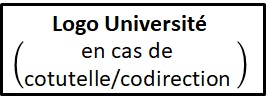
\includegraphics[width=5.5cm]{images/logo_cotut_codirec_latex.jpg} \hspace{6cm} 
\includegraphics[width=5.5cm]{images/Cnam.jpg}
\end{minipage}


\begin{minipage}{\textwidth}
\begin{center}
\vspace{1cm}
\textbf{Conservatoire national des arts et métiers} \\
\vspace{0.5cm}
\textbf{ÉCOLE DOCTORALE ABBÉ GRÉGOIRE} (supprimer la mention inutile) \\
\textbf{ÉCOLE DOCTORALE SCIENCES DES MÉTIERS DE L’INGÉNIEUR} (supprimer la mention inutile) \\
~\\
\vspace{0.1cm} 
\textbf{[Laboratoire de recherche]} 
\vspace{0.5cm} 
~\\
{\Huge \textbf{Thèse de doctorat}}
~\\
\vspace{0.5cm}
~\\
\text{Présentée par} : \textbf{Prénom NOM} \\
\vspace{0.1cm}
\text{Soutenue le} : \textbf{XX mois en lettres 20xx} \\
\vspace{0.1cm}
\text{Discipline} : \textbf{Section CNU à compléter} \\
\vspace{0.1cm}
\text{Spécialité} : \textbf{Spécialité à compléter} \\

\end{center}
\end{minipage}


\vspace{1cm}
\makebox[\textwidth][c]{
\fcolorbox{redHESAM}{white}{
\begin{minipage}{16.5cm}
\centering
\vspace{0.2cm}
{
~\\
{\LARGE\textbf{{TITRE DE LA TH\`ESE}}}
~\\
\vspace{0.4cm}
{\LARGE \textbf{[Sous-titre éventuel]}}
~\\}
%{\LARGE{\textbf{{}}}}
\vspace{0.2cm}
\end{minipage}
}
}
\vspace{0.8cm}


\begin{minipage}{\textwidth}
\begin{center}
\textbf{\textsc{\large TH\`{E}SE dirig\'{e}e par :}} \\
\vspace{0.1cm}
{\large \textbf{[Civilité Prénom NOM]}} {\large{Titre, Cnam}} \\
\vspace{0.5cm}
\textbf{\textsc{\large et co-encadrée/co-dirigée (supprimer la mention inutile) par :}} \\
{\large \textbf{[Civilité Prénom NOM]}} {\large{Titre, Cnam}} \\

\end{center}
\end{minipage}

\vspace{0.7cm}

\noindent 
\begin{minipage}{\textwidth}
\textbf{Jury} \\
   \begin{tabular}{p{5cm} p{5.5cm} l}
	 \textbf{Mme/M. Prénom NOM} & Titre, Unité de recherche, \'Ecole &  Président/Présidente  \\
	 \textbf{Mme/M. Prénom NOM} & Titre, Unité de recherche, \'Ecole &  Rapporteur/Rapportrice  \\
	 \textbf{Mme/M. Prénom NOM} & Titre, Unité de recherche, \'Ecole &  Rapporteur/Rapportrice  \\
	 \textbf{Mme/M. Prénom NOM} & Titre, Unité de recherche, \'Ecole &  Directeur de thèse/Directrice de thèse  \\
	 \textbf{Mme/M. Prénom NOM} & Titre, Unité de recherche, \'Ecole &  Co-directeur de thèse/Co-directrice de thèse\\
	 \textbf{Mme/M. Prénom NOM} & Titre, Unité de recherche, \'Ecole &  Co-directeur de thèse/Co-encadrante de thèse  \\
 	 \textbf{Mme/M. Prénom NOM} & Titre, Unité de recherche, \'Ecole & Examinateur/Examinatrice\\
     \textbf{Mme/M. Prénom NOM} & Titre, Unité de recherche, \'Ecole & Examinateur/Examinatrice\\
	 \textbf{Mme/M. Prénom NOM} & Titre, Unité de recherche, \'Ecole & Examinateur/Examinatrice \\
	 \textbf{Mme/M. Prénom NOM} & Titre, Unité de recherche, \'Ecole & Examinateur/Examinatrice \\
     \textbf{Mme/M. Prénom NOM} & Titre, Unité de recherche, \'Ecole & Examinateur/Examinatrice \\
     \textbf{Mme/M. Prénom NOM} & Titre, Unité de recherche, \'Ecole & Invité/Invitée
\end{tabular}  
\end{minipage}

%-----------Propriete du document ---------------------%

\thispagestyle{empty}

%-----------Definition des dimensions ------------------%

\setlength{\baselineskip}{1.5\baselineskip} %interligne de 1.5
\setlength{\voffset}{0pt} 				% offset vertical
\setlength{\topmargin}{0pt}				% Pas de marge en haut
\setlength{\headheight}{30pt}			% Haut de page
\setlength{\headsep}{30pt}				% Entre le haut de page et le texte
\setlength{\textheight}{620pt}		% Hauteur de la zone de texte
\setlength{\footskip}{30pt}				% Bas de page + séparation
\setlength{\hoffset}{-15pt} 				% offset horizontal
\setlength{\oddsidemargin}{0pt}	% Marge gauche sur pages impaires
\setlength{\evensidemargin}{0pt}	% Marge gauche sur pages paires
\setlength{\textwidth}{420pt}			% Largeur de la zone de texte 
\setlength{\marginparsep}{10pt}		% Séparation de la marge 10
\setlength{\marginparwidth}{40pt}	% Largeur de note dans la marge
\parskip=4pt									   % espace additionnel entre deux paragraphes

%--------------Style de page ---------------------------%

\pagestyle{fancy}


%--------------Page de dedicace------------------%

\newpage
\null
\newpage
\thispagestyle{empty}

\begin{flushright}
 Insérer éventuellement une dédicace ... 


\end{flushright}


%--------------Page de remerciement------------------%


\chapter*{Remerciements}
\addcontentsline{toc}{chapter}{Remerciements}
\adjustmtc
\markright{\MakeUppercase{Remerciements}}

 Insérer ici votre texte de remerciements

\noindent 

%--------------Page resume en fr ----------------------%

\begin{vcenterpage}

\chapter*{Résumé}
\addcontentsline{toc}{chapter}{Résumé}
\adjustmtc
\markright{\MakeUppercase{Resume}}

Insérer ici votre résumé en français suivi des mots-clés.\\

Mots-clés : mot-clé 1, mot-clé 2 , ... , mot-clé 10 (maximum) ...


\end{vcenterpage}

%--------------Page resume en en ----------------------%

\begin{vcenterpage}

\chapter*{Abstract}
\addcontentsline{toc}{chapter}{Abstract}
\adjustmtc
\markright{\MakeUppercase{Abstract}}

Insérer ici votre résumé en anglais.\\


Keywords : keyword 1, keyword 2, ... keyword 10 (maximum)...


\end{vcenterpage}

%--------------Les sommaires  ------------------------%


\tableofcontents
\listoftables            % à supprimer si pas de tableau
\addcontentsline{toc}{chapter}{Liste des tableaux}
\adjustmtc
\listoffigures           % à supprimer si pas de figure
\addcontentsline{toc}{chapter}{Liste des figures}
\adjustmtc

%--------------Introduction  ---------------------------%

%-  -%

%-  -%
\chapter*{Introduction}
\addcontentsline{toc}{chapter}{Introduction}
\adjustmtc
\markright{\MakeUppercase{Introduction}}

\newpage

Texte de l'introduction \\

Exemple bibliographie citation style numérique :

\begin{itemize}
\item[•] articles :  \cite{Zhou2015} et \cite{Patil2015,Eriksson2016}
\item[•] livre : \cite{Morand1995} 
\end{itemize}


%-------------- PARTIE 1 -------------------------------%

%\part{Titre de la première partie}

%-------------- CHAPITRE 1 ------------------------------%

\chapter{Titre du chapitre 1}
\minitoc   % mini sommaire facultatif

\newpage
\section{Titre de la section 1}
\subsection{Titre de la sous-section 1}
\subsubsection{Titre de la sous-sous-section 1}


%-------------- CHAPITRE 2 ------------------------------%

\chapter{Titre du chapitre 2}
\minitoc   % mini sommaire facultatif

\newpage
\section{Titre de la section 2}
\subsection{Titre de la sous-section 2}
\subsubsection{Titre de la sous-sous-section 2}



%-----------La  conclusion------------------------------%

\chapter*{Conclusion}
\addcontentsline{toc}{chapter}{Conclusion}
\adjustmtc
\markright{\MakeUppercase{Conclusion}}
\newpage

Texte de la conclusion. \\


%-----------La  biblio -----------------------------------%
\cleardoublepage\phantomsection
\addcontentsline{toc}{chapter}{Bibliographie}

\thispagestyle{empty}
\chapter*{Consigne bibliographie (à supprimer)} %  à supprimer
%\addcontentsline{toc}{chapter}{Consigne bibliographie}
%\markright{\MakeUppercase{Consigne bibliographie}}
%\adjustmtc

Rappel : qu’est-ce qu’une bibliographie ?
\begin{itemize}
\item une liste ordonnée de références de documents concernant un auteur ou un sujet.
\item permet l’identification claire des sources citées, présentées de manière ordonnée et conforme à des normes prescrites.
\end{itemize}

Le style de présentation de la bibliographie (ponctuation, majuscules,...) peut varier selon les disciplines et les documents. Il est à choisir avec la·le directeur·rice de thèse.
 
En Sciences humaines et sociales, privilégier un style de type « AUTEUR (date). TITRE » : comme les normes APA, Chicago ou Vancouver.
Dans le domaine de l’informatique et des sciences de l’ingénieur, privilégier le style IEEE : style numérique, par ordre d’apparition des références dans la thèse.
 
Une fois le style choisi, il devra être appliqué rigoureusement dans le travail de thèse pour toutes les références.
 
Recommandations : utiliser un logiciel de gestion de références bibliographiques tel que Zotero pour générer automatiquement la bibliographie et les citations tout au long de la thèse.
 
Des formations à Zotero sont dispensées par les bibliothèques du Cnam tout au long de l’année. Plus d’informations sur le site : https://bibliotheques.cnam.fr/, rubrique « Formation »\\

\newpage
\thispagestyle{empty}
\clearpage

%\bibliographystyle{alpha}
%\bibliographystyle{ieeetr}

\bibliographystyle{IEEEtran-francais}

%\bibliographystyle{plainnat}

%\printbibliography

\bibliography{biblio}
\thispagestyle{empty}


%-----------Les annexes -------------------------------%

\newpage
\appendix
\addcontentsline{toc}{chapter}{Liste des annexes}
\chapter{Titre de l'annexe A}
\markright{\MakeUppercase{Annexe A}}
\chapter{Titre de l'annexe B}
\markright{\MakeUppercase{Annexe B}}
\newpage

%----------- Le glossaire ---------------------------------%
%%----- Acronymes -----%

\newglossaryentry{usbl}{
     type=\acronymtype,
     name={USBL},
     description={système de positionnement acoustique par ligne de base ultra courte ou \emph{Ultra Short Base Line acoustic positioning system}},
     first={USBL (système de positionnement acoustique par ligne de base ultra courte ou \emph{Ultra Short Base Line acoustic positioning system})},
     }

\newglossaryentry{slam}{
     type=\acronymtype,
     name={SLAM},
     description={Localisation et cartographie simultanées ou \emph{Simultaneous Location And Mapping}},
     first={SLAM (Localisation et cartographie simultanées ou \emph{Simultaneous Location And Mapping})},
     }
     
\newglossaryentry{ascii}{
     type=\acronymtype,
     name={ASCII},
     description={Code américain normalisé pour l'échange d'information ou \emph{American Standard Code for Information Interchange}},
     first={ASCII (Code américain normalisé pour l'échange d'information ou \emph{American Standard Code for Information Interchange})},
     }
          
     
\newglossaryentry{lbl}{
     type=\acronymtype,
     name={LBL},
     description={système de positionnement acoustique par longue ligne de base ou \emph{Long BaseLine acoustic positioning system}},
     first={LBL (système de positionnement acoustique par longue ligne de base ou \emph{Long BaseLine acoustic positioning system})},
     }
     
\newglossaryentry{auv}{
     type=\acronymtype,
     name={AUV},
     description={Véhicule sous-marin autonome ou \emph{Autonomous Underwater Vehicle}},
     first={AUV (Véhicule sous-marin autonome ou \emph{Autonomous Underwater Vehicle})},     
     }
     
\newglossaryentry{uuv}{
     type=\acronymtype,
     name={UUV},
     description={Véhicule sous-marin non-habité ou \emph{Unmanned Underwater Vehicle}},
     first={UUV (Véhicule sous-marin non-habité ou \emph{Unmanned Underwater Vehicle})},     
     }
     
\newglossaryentry{rov}{
     type=\acronymtype,
     name={ROV},
     description={Véhicule téléguidé ou \emph{Remotely Operated Vehicle}},
     first={ROV (Véhicule téléguidé ou \emph{Remotely Operated Vehicle})},     
     }
     
\newglossaryentry{hrov}{
     type=\acronymtype,
     name={HROV},
     description={Véhicule téléguidé hybride ou \emph{Hybrid Remotely Operated Vehicle}},
     first={HROV (Véhicule téléguidé hybride ou \emph{Hybrid Remotely Operated Vehicle})},     
     }
     
\newglossaryentry{gravimob}{
    type=\acronymtype,
    name={GraviMob},
    description={Système de Gravimétrie Mobile ou \emph{Mobile Gravimetry System}},
    first={GraviMob (Système de Gravimétrie Mobile ou \emph{Mobile Gravimetry System})},
    }
    
\newglossaryentry{limog}{
    type=\acronymtype,
    name={LiMo-g},
    description={Système Léger de Gravimétrie Mobile ou \emph{Light Moving Gravimetry System}},
    first={LiMo-g (Système Léger de Gravimétrie Mobile ou \emph{Light Moving Gravimetry System})},
    }
    
\newglossaryentry{ldo}{
    type=\acronymtype,
    name={LDO},
    description={Laboratoire de Domaines Océaniques},
    first={LDO (Laboratoire de Domaines Océaniques)},
    }
    
\newglossaryentry{ifremer}{
    type=\acronymtype,
    name={IFREMER},
    description={Institut Français de Recherche pour l'Exploitation de la Mer},
    first={Institut Français de Recherche pour l'Exploitation de la Mer (IFREMER)},
    }
    
\newglossaryentry{ipgp}{
    type=\acronymtype,
    name={IPGP},
    description={Institut de Physique du Globe de Paris},
    first={Institut de Physique du Globe de Paris (IPGP)},
    }

\newglossaryentry{onera}{
    type=\acronymtype,
    name={ONERA},
    description={Office National d'Études et de Recherches Aérospatiales},
    first={Office National d'Études et de Recherches Aérospatiales (ONERA)},
    }

\newglossaryentry{shom}{
    type=\acronymtype,
    name={SHOM},
    description={Service Hydrographique et Océanographique de la Marine},
    first={Service Hydrographique et Océanographique de la Marine (SHOM)},
    }    
    
\newglossaryentry{grs80}{
    type=\acronymtype,
    name={GRS80},
    description={Système de Référence Géodésique 1980 ou \emph{Geodetic Reference System 1980}},
    }
    
\newglossaryentry{svd}{
    type=\acronymtype,
    name={SVD},
    description={Décomposition en Valeurs Singulières ou \emph{Singular Value Decomposition}},
    first={décomposition en valeurs singulières ou \emph{Singular Value Decomposition} (SVD)},
    }   

\newglossaryentry{esgt}{
    type=\acronymtype,
    name={ESGT},
    description={École Supérieure des Géomètres et Topographes},
    first={École Supérieure des Géomètres et Topographes~(ESGT)},
    } 
    
\newglossaryentry{egm08}{
    type=\acronymtype,
    name={EGM2008},
    description={\emph{Earth Gravitational Model 2008}},
    first={EGM2008 (\emph{Earth Gravitational Model 2008})},
    } 

\newglossaryentry{odp}{
    type=\acronymtype,
    name={OP},
    description={Observatoire de Paris},
    first={Observatoire de Paris (OP)},
    } 

\newglossaryentry{ign}{
    type=\acronymtype,
    name={IGN},
    description={Institut National de l'information Géographique et forestière},
    first={Institut National de l'information Géographique et forestière (IGN)},
    } 

\newglossaryentry{lareg}{
    type=\acronymtype,
    name={LAREG},
    description={Laboratoire de Recherche en Géodésie},
    first={Laboratoire de Recherche en Géodésie (LAREG)},
    } 
    
\newglossaryentry{gps}{
    type=\acronymtype,
    name={GPS},
    description={Système Global de Positionnement ou \emph{Global Positioning System}},
    first={GPS (Système Global de Positionnement ou \emph{Global Positioning System})},
    } 
    
\newglossaryentry{mems}{
    type=\acronymtype,
    name={MEMS},
    description={Microsystème électromécanique ou \emph{Microelectromechanical systems}},
    first={MEMS (Microsystème électromécanique ou \emph{Microelectromechanical systems})},
    } 
%----- Définition -----%

\newglossaryentry{i-frame}{
	name={\emph{i-frame}},
	description={le \emph{i-frame} (ou \emph{inertial-frame}) désigne le repère accompagnant la Terre dans son mouvement de translation elliptique autour du Soleil},
	}    

\newglossaryentry{e-frame}{
	name={\emph{e-frame}},
	description={le \emph{e-frame} (ou \emph{earth-frame}) désigne le repère accompagnant la Terre dans son mouvement de rotation sur elle-même},
	} 

\newglossaryentry{n-frame}{
	name={\emph{n-frame}},
	description={le \emph{n-frame} (ou \emph{navigation-frame}) désigne le repère géographique local},
	first={\emph{n-frame}},
	}    
    
\newglossaryentry{b-frame}{
	name={\emph{b-frame}},
	description={le \emph{b-frame} (ou \emph{body-frame}) désigne le repère attaché au véhicule porteur},
	first={\emph{b-frame}},
	}

\newglossaryentry{alpha-frame}{
	name={$s_{\alpha}$\emph{-frame}},
	description={le $s_{\alpha}$\emph{-frame} (resp. $s_{\beta}$\emph{-frame}) (ou \emph{system-frame}) est le repère attaché à la triade accélérométrique $\alpha$ (resp. $\beta$)},
	first={$s_{\alpha}$\emph{-frame}},
	}
	
\newglossaryentry{beta-frame}{
	name={$s_{\beta}$\emph{-frame}},
	description={le $s_{\alpha}$\emph{-frame} (resp. $s_{\beta}$\emph{-frame}) (ou \emph{system-frame}) est le repère attaché à la triade accélérométrique $\alpha$ (resp. $\beta$)},
	first={$s_{\beta}$\emph{-frame}},
	}

%----- Symboles -----%     
     
\newglossaryentry{delta}{
     type=notation,
     name={\ensuremath{\delta}},
    description={Angle de cap},
    sort={delta}
     }




%\printglossary[type=\acronymtype, title={Liste des acronymes}, toctitle={Liste des acronymes}]
%\printglossary[title=Glossaire, toctitle=Glossaire]
%\printglossary[type=notation, title={Liste des symboles}, toctitle={Liste des symboles}]


%======== FIN DU DOCUMENT ================%
\end{document}